%\documentclass{cumcmthesis}
    \documentclass[withoutpreface,bwprint]{cumcmthesis} %去掉封面与编号页

    \title{龙门吊问题的数学建模}
    \tihao{A}            % 题号
    \baominghao{042}    % 报名号
    \schoolname{武汉大学}
    \membera{周澳}
    \memberb{傅宇千}
    \memberc{刘志豪}
    \supervisor{指导老师}
    \yearinput{2020}     % 年
    \monthinput{08}      % 月
    \dayinput{15}        % 日

\begin{document}
\maketitle
\begin{abstract}
    对于港口装卸货物集装箱的龙门吊的吊运过程的求解与优化问题,本文通过建立货物运动的动力学模型,以及对摆角、效率的优化模型进行求解。首先,对于货物在吊运过程中的运动问题,由于这是一种完整约束下的具有一个自由度的平面运动,可以通过使用分析力学中的拉格朗日方程,解出在吊车处于4段不同运动状态下的货物的以摆角$\theta$为广义坐标的运动微分方程。使用Matlab软件数值求解微分方程可以得到货物在吊运过程中的运动状态。

    对于前三问提出的不同的优化问题,我们可以通过不同的优化方法解出针对各问题的较优解。对于第一问仅对在岸上运动的最大摆角进行优化的问题,我们使用多起点寻找局部最小值的方法搜索可行的较优解,并取了其中摆角最小的一个作为答案:当$(t_1,t_2,t_3,t_4)=(5.57s,15.97s,5.2s,93.02s)$时,货物在BC段的最大摆角$\theta_{max}=0.54^{\circ}$。第二问在第一问的基础上增加了对吊运效率的考虑,由于货物质量固定,我们把效率看作吊运时间,通过对第一问搜出的许多局部较优解使用逼近理想解排序(TOPSIS)法和熵权法确定其中的较优解,我们得到的一组较优解为:$(t_1,t_2,t_3,t_4)=(5.57s,16.00s,5.08s,61.25s),\quad \theta_{max}=0.96^{\circ},t=87.9s$。

    第四问要求设计一个可以直观演示吊运过程的图形界面,我们通过使用Matlab的图形界面设计工具,设计了一个能够在给定$a,t_i$的情况下给出货物的运动演示图的图形窗口。

    \keywords{分析力学\quad  微分方程数值求解\quad   多起点优化\quad 遗传算法\quad GUI演示设计}
\end{abstract}
%\tableofcontents
\section{问题重述}
%\subsection{问题的提出}
某公司一货运码头,配备带有动力驱动的货运吊车。现需将货物从货运船的起吊点吊运到货运码头的终点,并且按照规定的方式进行运动,提出如下问题:

(1)在不考虑吊车缆绳承载力的情况下,确定吊车运行方式,即建立模型,确定时间的大小,使得货物从岸边到终点,其间摆动最小,且整个吊运时间不超过2分钟;

(2)在第一问条件下,如果同时计及吊运效率,建立模型确定时间的大小,使货物从岸边到终点 不仅摆动幅度小而且整体效率高;

(3)考虑缆绳的最大承载力,并兼顾摆动大小和效率,请建立模型,确定吊车运行方式,即确定加速度的大小、时间,并确定最大起吊货物重量;

(4)考虑实际问题的需要,为该公司设计一套图形计算机演示系统,直观演示龙门吊吊运过程。
\section{符号说明}
\begin{center}
    \begin{tabular}{cc}
        \hline
        \makebox[0.3\textwidth][c]{符号} & \makebox[0.4\textwidth][c]{意义}        \\ \hline
        $a$                              & 吊车加速度大小($m/s^{-2}$)              \\ \hline
        $g$                              & 重力加速度,$9.8m/s^{-2}$               \\ \hline
        $x(t),y(t)$                      & 货物在时刻$t$的位置坐标                 \\ \hline
        $v_x(t),v_y(t)$                  & 货物在时刻$t$的水平、竖直速度           \\ \hline
        $\theta(t)$                      & 吊绳在时刻$t$与竖直方向夹角,顺时针为正 \\ \hline
        $\theta_{max}$                   & 从B点到C点货物运动过程中的最大摆角      \\ \hline
        $v_{4xmax}$                      & 货物到终点处的水平速度                  \\ \hline
        $x_a(t),v_a(t)$                  & 吊车在时刻$t$时的位置坐标,运动速度     \\ \hline
        $t_{1,2,3,4}$                    & 第1-4段运动分别持续的时间$(s)$          \\ \hline
        $T_i,i=1,2,3,4$                  & 第$i$段运动结束的时刻$(s)$              \\ \hline
        $F(t)$                           & 吊绳在时刻$t$时的拉力大小$(N)$          \\ \hline
        $F_{max}$   & 吊绳的最大拉力,值为$20000g\quad N$ \\ \hline
    \end{tabular}
\end{center}
\section{问题分析}
题目给出的龙门吊问题可以看作二维的质点运动问题,因为吊车只沿直线运动,货物没有初速度,在吊车前进的过程中货物只会在包含吊车运动轨迹的与地面垂直的平面内运动。货物的运动也不是平面内的自由运动,而是受到了来自吊车和吊绳的约束,因此货物的运动自由度实际上只有一个,可以用吊绳与竖直方向的夹角$\theta$表示。由于货物的运动受到的约束是完整约束,可以使用分析力学中的拉格朗日方程可以解出其运动微分方程,微分方程可以用软件进行数值求解,这样可以建立货物运动的动力学模型,可以在给定所有参数时解出整个过程的运动状态。

前三问是在不同的参数、目标下的优化问题,可以使用优化模型求解。第一问在加速度给定时仅要求对货物的摆动角度进行优化,第二问在第一问的基础上同时要对整个过程的效率进行优化,第三问比第二问增加了加速度这一参数,并且要求给出能够吊运货物的最大质量。首先考虑效率的定义,由于写出的运动微分方程与货物的质量无关,在相同的吊运方式下,货物质量仅仅受到吊绳能够承受的最大拉力的限制,因此我们认为效率只与时间相关,吊运时间越短效率越高。我们可以根据运动的动力学模型写出最大摆角、吊运时间和实际吊绳最大拉力与$t_{1,2,3,4}$的程序函数,然后通过调用不同的优化算法来求解不同的优化问题。对于较为简单的前两问,可以使用多起点搜索最小值的方法;对于第三问,可以使用遗传算法、退火算法等优化算法进行求解。

对于第四问要求的设计展示龙门吊吊运过程的图形界面(GUI),我们可以使用matlab的图形设计工具进行设计。

\section{模型假设}
\begin{enumerate}
    \item 把货物当作质点;
    \item 货物只做平面运动;
    \item 吊绳的质量忽略不计;
    \item 货物摆动过程中不计各种阻力;
    \item 整个过程中吊绳始终处于拉紧状态,且长度不变;
    \item 吊运的效率仅取决于吊运过程耗费的时间;
    \item 吊车到达终点后会立刻刹车将速度降至0。
\end{enumerate}

\section{建立模型}
\subsection{货物运动的动力学模型}
如图所示建立坐标系:

\centerline{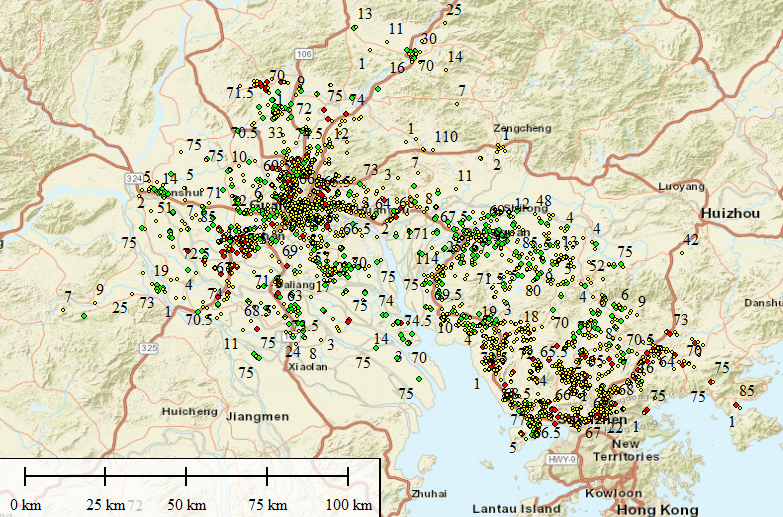
\includegraphics[width=10cm]{1.png}}
设吊车位置坐标为$x_a$,速度为$v_a$;货物的位置$(x,y)$,速度$v$,水平速度$v_{x}$,缆绳与竖直方向的角度为$\theta$(顺时针为正)。令$T_1=t_1,\quad T_2=t_1+t_2,\quad T_3=t_1+t_2+t_3,\quad T_4=t_1+t_2+t_3+t_4$。吊绳能承受的最大拉力$T_{max}=20000g,\quad g$取$9.8m/s^2$。$AB$间距离为$D_1$,$CD$间距离为$D_2$。

取货物为研究对象,用分析力学方法,取广义坐标$\theta$

(1)当$0 \leq t \leq T_1$时,吊车匀加速运动,对于货物有如下拉格朗日函数:
$$L_{1}=\frac{m}{2}\left(l^{2} \dot{\theta}^{2}-2 a l \dot{\theta} t \cos \theta+a^{2} t^{2}\right)+m gl\cos \theta$$

代入拉格朗日方程$$\frac{d}{d t}\left(\frac{\partial L_{1}}{\partial \dot{\theta}}\right)-\frac{\partial L_1}{\partial \theta}=0$$

得到运动微分方程:$$l \ddot{\theta}+a \dot{\theta} t \sin \theta-a \cos \theta+g \sin \theta=0$$
$$\text{初始条件}\left.\theta\right|_{t=0}=0,\left.\quad \dot{\theta}\right|_{t=0}=0$$

由$\theta(t),0 \leqslant t \leqslant T_{1}$,有

$$\left\{\begin{array}{l}
        x=x_{a}-l \theta \sin \theta=\frac{a}{2} t^{2}-\operatorname{lsim} \theta \\
        v_{x}=v_{a}-l \dot{\theta} \cos \theta=a t-l \dot{\theta} \cos \theta
    \end{array}\right.$$

(2)当$T_1 \leq t \leq T_2$时,吊车匀速运动,对于货物同上可得运动微分方程:
$$l\ddot{\theta}-v_{a2}\dot{\theta}\sin\theta+(v_{a2}+g) \sin \theta=0$$
$$\text{初始条件}\left \{\begin{array}{l}
        \left.\theta\right|_{t=T_{1}^{+}}=\left.\theta\right|_{t=T_{1}^{-}} \\
        \left.\dot{\theta}\right|_{t=T_{1}^{+}}=\left.\dot{\theta}\right|_{t=T_{1}^{-}}
    \end{array}\right.$$

此时有:$$\left\{\begin{array}{l}
        x=x_{a}-l\theta \sin \theta=\frac{a}{2} T_{1}^{2}+aT_1(t-T_1)-l\sin \theta \\
        v_{x}=v_{a}-l \dot{\theta} \cos \theta=a T_{1}-l\dot{\theta }\cos \theta
    \end{array}\right.$$

(3)当$T_2 \leq t \leq T_3$时,吊车匀减速运动,对于货物同(1)可得运动微分方程:
$$l \ddot{\theta}+a\left(T_{1}+T_{2}-t\right) \dot{\theta} \sin \theta+a \cos \theta+g \sin \theta=0$$
$$\text{初始条件}\left \{\begin{array}{l}
        \left.\theta\right|_{t=T_{2}^{+}}=\left.\theta\right|_{t=T_{2}^{-}} \\
        \left.\dot{\theta}\right|_{t=T_{2}^{+}}=\left.\dot{\theta}\right|_{t=T_{2}^{-}}
    \end{array}\right.$$
此时有:$$\left\{\begin{array}{l}
        v_{x}=a\left(T_{1}+T_{2}-t\right)-l \dot{ \theta} \cos \theta \\
        x=x_{2}+aT_{1}(t-T_{2})-\frac{a}{2}(t-T_{2})^{2}-l\sin\theta
    \end{array}\right.$$
并且需要满足在匀减速运动结束时吊车刚好到达B点,即$$\frac{a}{2}t_1^2+at_1t_2+\frac{a}{2}t_3(2t_1-t_3)=D_1$$

(4)当$T_3 \leq t \leq T_4$时,吊车匀速运动,对于货物同(1)可得运动微分方程:
$$l\ddot{\theta}-v_{a4}\dot{\theta}\sin\theta+(v_{a4}+g) \sin \theta=0$$
%$$\ddot{\theta}+\frac{g}{l} \sin \theta=0$$
$$\text{初始条件}\left \{\begin{array}{l}
        \left.\theta\right|_{t=T_{3}^{+}}=\left.\theta\right|_{t=T_{3}^{-}} \\
        \left.\dot{\theta}\right|_{t=T_{3}^{+}}=\left.\dot{\theta}\right|_{t=T_{3}^{-}}
    \end{array}\right.$$
此时有:$$\left\{\begin{array}{l}
        v_{x}=a\left(T_1+T_{2}-T_{3}\right)-l \dot{\theta} \cos \theta \\
        x=D_1+a\left(T_{1}+T_{2}-T_{3}\right)\left(t-T_{3}\right)-l \sin \theta
    \end{array}\right.$$

从B点到C点货物运动过程中的最大摆角$\theta_{\max }=\max \theta(t), \quad T_3 \leqslant t \leqslant T_{4}$,

对于货物最终的水平速度,取第四段匀速过程中货物水平速度绝对值的最大值$v_{4xmax}=max\left \{v_{x},T_3 \leq t \leq T_4\right \}$,要求$v_{4xmax} \leq 0.5m/s$。

运动全过程中货物的竖直速度$v_{y}=-l\dot{\theta}\sin\theta,\quad 0\leq t\leq T_4$,对速度求导可得水平、竖直方向的加速度,由此可以计算整个运动过程中每一时刻的拉力:$$\left\{\begin{array}{l}
        F_{x}=m a_{x}   \\
        F_{y}=mg-ma_{y} \\
        F=\sqrt{F_{x}^2 + F_{y}^2}
    \end{array}\right.$$
要求$F \leq F_{max},0 \leq t \leq T_4$

\subsection{对摆角、效率的优化模型}
\subsubsection{仅考虑摆角的优化模型}
针对第一问提出的问题,在加速度确定的情况下,考虑到题目中对运动的限制,即在匀减速运动结束时吊车要正要运动到B点:$$x_{a1}+x_{a2}+x_{a3}=\frac{a}{2}t_1^2+at_1t_2+\frac{a}{2}t_3(2t_1-t_3)=D_1$$可以把参数$t_{1,2,3,4}$简化为只需要两个参数$t_1,t_3$。通过上节建立的动力学模型可以求出在BC段运动过程中的最大摆角$\theta_{max}$。由此可以建立单目标优化模型如下:
$$min\quad \theta_{max}$$
$$\text{$s.t.$}\left \{\begin{array}{l}
        v_{4xmax}<0.5m/s \\
        T_4\leq120s      \\
        F<F_{max},0\leq t\leq T_4
    \end{array}\right.$$

\subsubsection{考虑摆角、效率的优化模型}

第二问在第一问的基础上同时考虑BC段的最大摆角$\theta_{max}$和吊运效率的,优化模型由单目标变为多目标。由于该问题中的货物质量固定为$m=6000kg$,我们便把效率定义为时间的线性函数,吊运所用的总时间越短,调运效率越高。在用第一问的方法已经求得若干有不同的BC段最大摆角、吊运时间的解的情况下,可以通过逼近理想解排序模型(TOPSIS)找出相对较优的一种解。我们可以首先找到所有解当中摆角$\theta_{max}$和时间$t$的最大值与最小值,使用极差标准化方法得到这若干种情形下的摆角和时间的效益型属性值,取理想解为两属性都取最小值,负理想解为两属性都取最大值,调整两个目标的权重$w_1,w_2$,解出每种情形下与理想解的贴近度$\frac{d^+}{d^++d^-}$,取与最理想解最贴近近的解作为该问题的答案。

\subsubsection{考虑加速度时对摆角、效率的优化模型}
对于第三问提出的问题,自变量比前两问增加了一个加速度$a, 0<a\leq1$,而优化目标和第二问相同,仍是$\theta_{max}$和$t$。

\section{模型求解}
我们首先将货物运动的动力学模型使用matlab编写为一个函数脚本,其中四段运动过程的常微分方程使用ode45求解器进行数值求解,当给定的参数$a,t1,t3$满足题目中的限制要求,则计算出这种运动样式下的最大摆角和吊运时间,否则返回一个设定的极大值。我们针对前三问不同的优化目标对函数脚本进行对应的修改,以满足不同的求解需求。函数脚本func.m见附录。

\subsection{第一问的求解}
考虑到动力学模型的最大摆角——$(t_1,t_3)$不是线性关系,在特定区间的取值由于不满足模型限制而返回极大值,因此很难通过一次简单的优化过程找到最优解。为此我们使用了在多个起点运行区域极小值的搜索函数,具体而言是使用了matlab的fminsearch函数,在$t_1=[3,12],\quad t_3=[t_1-2,t_1]$的范围均匀取初始点多次运行,找到若干局部较优解,再从中取$\theta_{max}$最小的解作为最终解。运行后得到当$(t_1,t_2,t_3,t_4)=(5.57s,15.97s,5.2s,93.02s)$时,货物在BC段的最大摆角$\theta_{max}=0.54^{\circ}$。这种情况下的货物$\theta(t),x(t)$曲线如下图所示。(不同颜色的线条代表4段不同的运动过程)
\begin{figure}[!h]
    \centering
    \begin{minipage}[c]{0.48\textwidth}
        \centering
        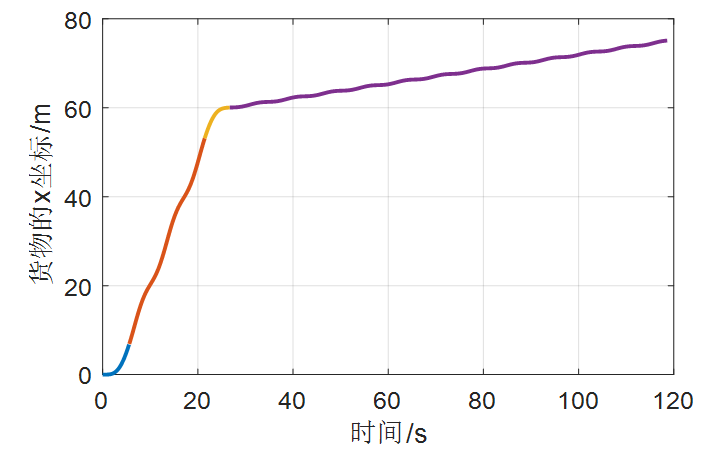
\includegraphics[width=\textwidth]{p1x.png}
        %\subcaption{时间-x坐标图像}
        \label{fig:sample-figure-a}
    \end{minipage}
    \begin{minipage}[c]{0.48\textwidth}
        \centering
        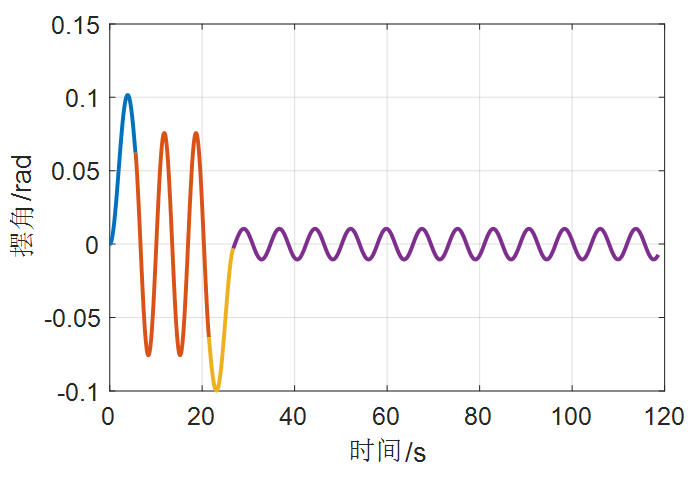
\includegraphics[width=\textwidth]{p1theta.png}
        %\subcaption{时间-摆角图像}
        \label{fig:sample-figure-b}
    \end{minipage}
    \caption{问题一解的$\theta(t)\quad x(t)$图像}
    \label{fig:sample-figure}
\end{figure}

\subsection{第二问的求解}
第二问在第一问的基础上增加了对吊运效率的考虑,也就是使吊运时间越短越好。为此,我们采取了先找出最大摆角接近第一问解得的最小值的若干解,再对这些解的摆角和时间使用逼近理想解排序法进行排序,取结果最好的一个作为问题的解。我们使用第一问的程序找出所有BC段最大摆角小于$1.89^{\circ}$的解,即找到$\theta_{max}$在三倍最小值的范围内的所有解,共得到了30组解,观察发现其中摆角最大的是$1.43^{\circ}$,且其用时为两分钟;其余的解都要比这个更好;我们又发现在所有的解当中,用时最短的是$82.14s$。因此我们以最小值$\theta_{max}=0.63^{\circ},t=82.14s$,和最大值$\theta_{max}=1.43^{\circ},t=120s$使用极差标准化解出每种解的效益性指标属性值$a_{\theta i}=\frac{\theta_i-0.63^{\circ}}{1.43^{\circ}-0.63^{\circ}},\quad a_{ti}=\frac{t_i-82.14s}{120s-82.14s}$。令理想解为两属性值都取最小值,负理想解为两属性值都取最大值。取对摆角和时间的权值分别为$(w_{\theta},w_t)=(0.6,0.4),(0.5,0.5),(0.7,0.3)$三种权值组合,求得每组解与理想解与负理想解的加权欧氏距离$d^+,d^-$,最后得到每组解与理想解的贴近度$c_i=\frac{d^-}{d^++d^-}$,对其排序后得到贴近度最大的一组解如下:
$$(t_1,t_2,t_3,t_4)=(5.57s,16.00s,5.08s,61.25s),\quad \theta_{max}=0.96^{\circ},t=87.9s$$。
该吊运过程的$\theta(t),x(t)$曲线如下图所示。
\begin{figure}[!h]
    \centering
    \begin{minipage}[c]{0.48\textwidth}
        \centering
        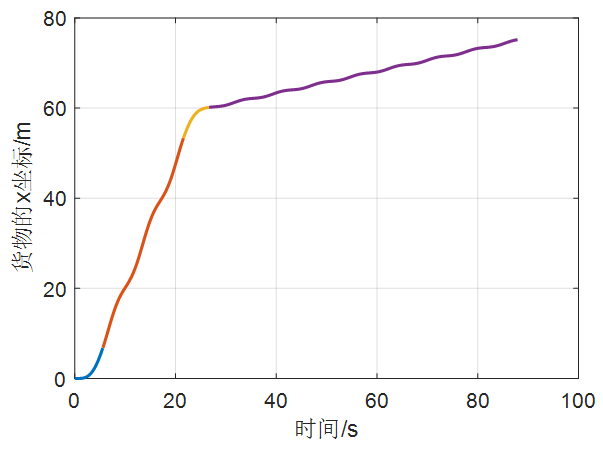
\includegraphics[width=\textwidth]{p2x.png}
        %\subcaption{时间-x坐标图像}
        \label{fig:sample-figure-a}
    \end{minipage}
    \begin{minipage}[c]{0.48\textwidth}
        \centering
        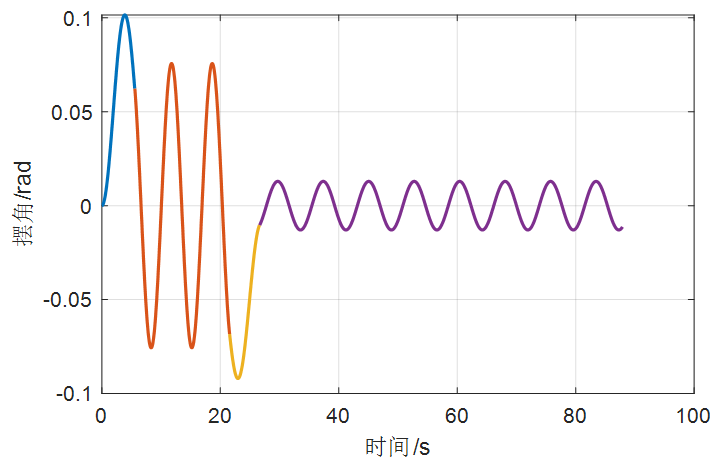
\includegraphics[width=\textwidth]{p2theta.png}
        %\subcaption{时间-摆角图像}
        \label{fig:sample-figure-b}
    \end{minipage}
    \caption{问题二解的$\theta(t)\quad x(t)$图像}
    \label{fig:sample-figure}
\end{figure}

\section{模型检验}
\section{总结与推广}
\begin{thebibliography}{9}%宽度9
    \bibitem{bib:one} ....
\end{thebibliography}
\begin{appendices}
    \section{MATLAB源程序1}

    \begin{lstlisting}[language=matlab]
        function [Time, Angle, Mmax]=func(a,t1,t3)
        inf=10000000;
        D1=60; D2=15; l=15; m=6000;
        g=9.8; Tmax=20000*g;
        %a=0.5; t1=5; t2=20; t3=4;%此时t为每段的时间间隔
        xa1=a*t1*t1/2; xa3=D1; xa4=D1+D2; xa2=xa3-0.5*a*t3*(2*t1-t3);
        t2=(xa2-xa1)/(a*t1); t4=(xa4-xa3)/(a*(t1-t3)); %xai为第i段结束后吊车的位移
        t2=t2+t1; t3=t2+t3; t4=t3+t4;%此时t为每段结束的时刻
        t=cell(4,1); theta=cell(4,1); x=cell(4,1); y=cell(4,1); %时间,角度,横纵坐标
        va=cell(4,1); va{2}=a*t1; va{4}=a*(t1+t2-t3);%吊车速度
        v=cell(4,1); Tx=cell(4,1); Ty=cell(4,1); T=cell(4,1); %水平速度,拉力,
        ax=cell(4,1); ay=cell(4,1);%水平竖直加速度
        thetamax=0; Tm=0; %实际最大的角度,拉力
        
        if t2<0 || (t3-t2)>=t1 || (t2-t1)<0.1 || t4>120
            Time=inf; Angle=inf; Mmax=inf;
            return;
        end
        
        %第一段加速
        dydt=@(t,y)[ y(2) ; (-a*y(2)*t*sin(y(1))+a*cos(y(1))-g*sin(y(1)))/l ];
        options = odeset('RelTol',1e-5,'AbsTol',[1e-5 1e-5]);
        [t{1},theta{1}] = ode45(dydt,[0:0.01:t1],[0 0],options);
        x{1}=0.5*a*t{1}.^2-l*sin(theta{1}(:,1));
        v{1}=a*t{1}-l*theta{1}(:,2).*cos(theta{1}(:,1));
        
        %第二段匀速
        dydt=@(t,y)[ y(2) ; (1/l)*(va{2}*y(2)*sin(y(1))-(va{2}+g)*sin(y(1))) ];
        options = odeset('RelTol',1e-5,'AbsTol',[1e-5 1e-5]);
        [t{2},theta{2}] = ode45(dydt,[t1:0.01:t2],[theta{1}(length(theta{1}(:,1)),1) theta{1}(length(theta{1}(:,2)),2)],options);
        x{2}=xa1+a*t1*(t{2}-t1)-l*sin(theta{2}(:,1));
        v{2}=a*t1-l*theta{2}(:,2).*cos(theta{2}(:,1));
        
        %第三段减速
        dydt=@(t,y)[ y(2) ; (-a*y(2)*(t1+t2-t)*sin(y(1))-a*cos(y(1))-g*sin(y(1)))/l ];
        options = odeset('RelTol',1e-5,'AbsTol',[1e-5 1e-5]);
        [t{3},theta{3}] = ode45(dydt,[t2:0.01:t3],[theta{2}(length(theta{2}(:,1)),1) theta{2}(length(theta{2}(:,2)),2)],options);
        x{3}=xa2+a*t1*(t{3}-t2)-0.5*a*(t{3}-t2).^2-l*sin(theta{3}(:,1));
        v{3}=a*(t1+t2-t{3})-l*theta{3}(:,2).*cos(theta{3}(:,1));
        
        %第四段匀速
        dydt=@(t,y)[ y(2) ; (1/l)*(va{4}*y(2)*sin(y(1))-(va{4}+g)*sin(y(1))) ];
        options = odeset('RelTol',1e-5,'AbsTol',[1e-5 1e-5]);
        [t{4},theta{4}] = ode45(dydt,[t3:0.01:t4],[theta{3}(length(theta{3}(:,1)),1) theta{3}(length(theta{3}(:,2)),2)],options);
        x{4}=xa3+a*(t1+t2-t3)*(t{4}-t3)-l*sin(theta{4}(:,1));
        v{4}=a*(t1+t2-t3)-l*theta{4}(:,2).*cos(theta{4}(:,1));
        thetamax=max(theta{4}(:,1));
        
        for i=1:4
            y{i}=l*cos(theta{i}(:,1));
            ax{i}=gradient(v{i},0.05);
            Tx{i}=m*ax{i};
            ay{i}=-1*(gradient(theta{i}(:,2),0.05).*sin(theta{i}(:,1)) + cos(theta{i}(:,1)).*theta{i}(:,2).^2);
            Ty{i}=m*(g-l*ay{i});
            T{i}=(Tx{i}.^2 + Ty{i}.^2).^0.5;
            Tm=max(Tm,max(T{i}));
            p=plot(x{i},-y{i},'linewidth',1.5);
            hold on;
        end
        
        E4 = 0.5*m*(v{4}(length(v{4}))^2 + (l*theta{4}(length(theta{4}(:,2)),2)*sin(theta{4}(length(theta{4}(:,1)),1)))^2);
        vcx=(2*E4/m + 2*g*l*(1-cos(theta{4}(length(theta{4}(:,1)),1))))^0.5;
        thetamax=max(thetamax,acos(1-E4/(m*g*l)));
        
        vcx=max(vcx,max(v{4}));
        if Tm>Tmax || vcx>0.5 %若拉力超限,最终速度超限
            Time=inf; Angle=inf;
            return;
        end
        
        Time=t4; Angle=thetamax; Mmax=m*Tmax/Tm;
     \end{lstlisting}
    \section{MATLAB源程序2}
    \begin{lstlisting}[language=matlab]
        function Angle=func1(input)
inf=10000000;
D1=60; D2=15; l=15; m=6000;
g=9.8; Tmax=20000*g; 
a=0.5; t1=input(1); t3=input(2);%此时t为每段的时间间隔
xa1=a*t1*t1/2; xa3=D1; xa4=D1+D2; xa2=xa3-0.5*a*t3*(2*t1-t3);
t2=(xa2-xa1)/(a*t1); t4=(xa4-xa3)/(a*(t1-t3)); %xai为第i段结束后吊车的位移
t2=t2+t1; t3=t2+t3; t4=t3+t4;%此时t为每段结束的时刻
t=cell(4,1); theta=cell(4,1); x=cell(4,1); y=cell(4,1); %时间,角度,横纵坐标
va=cell(4,1); va{2}=a*t1; va{4}=a*(t1+t2-t3);%吊车速度
v=cell(4,1); Tx=cell(4,1); Ty=cell(4,1); T=cell(4,1); %水平速度,拉力,
ax=cell(4,1); ay=cell(4,1);%水平竖直加速度
thetamax=0; Tm=0; %实际最大的角度,拉力

if t2<0 || (t3-t2)>=t1 || (t2-t1)<0.1 || t4>120
    Time=inf; Angle=inf; Tm=inf;
    return;
end

%第一段加速
dydt=@(t,y)[ y(2) ; (-a*y(2)*t*sin(y(1))+a*cos(y(1))-g*sin(y(1)))/l ];
options = odeset('RelTol',1e-5,'AbsTol',[1e-5 1e-5]);
[t{1},theta{1}] = ode45(dydt,[0:0.05:t1],[0 0],options);
x{1}=0.5*a*t{1}.^2-l*sin(theta{1}(:,1));
v{1}=a*t{1}-l*theta{1}(:,2).*cos(theta{1}(:,1));

%第二段匀速
dydt=@(t,y)[ y(2) ; (1/l)*(va{2}*y(2)*sin(y(1))-(va{2}+g)*sin(y(1))) ];
options = odeset('RelTol',1e-5,'AbsTol',[1e-5 1e-5]);
[t{2},theta{2}] = ode45(dydt,[t1:0.05:t2],[theta{1}(length(theta{1}(:,1)),1) theta{1}(length(theta{1}(:,2)),2)],options);
x{2}=xa1+a*t1*(t{2}-t1)-l*sin(theta{2}(:,1));
v{2}=a*t1-l*theta{2}(:,2).*cos(theta{2}(:,1));

%第三段减速
dydt=@(t,y)[ y(2) ; (-a*y(2)*(t1+t2-t)*sin(y(1))-a*cos(y(1))-g*sin(y(1)))/l ];
options = odeset('RelTol',1e-5,'AbsTol',[1e-5 1e-5]);
[t{3},theta{3}] = ode45(dydt,[t2:0.05:t3],[theta{2}(length(theta{2}(:,1)),1) theta{2}(length(theta{2}(:,2)),2)],options);
x{3}=xa2+a*t1*(t{3}-t2)-0.5*a*(t{3}-t2).^2-l*sin(theta{3}(:,1));
v{3}=a*(t1+t2-t{3})-l*theta{3}(:,2).*cos(theta{3}(:,1));

%第四段匀速
dydt=@(t,y)[ y(2) ; (1/l)*(va{4}*y(2)*sin(y(1))-(va{4}+g)*sin(y(1))) ];
options = odeset('RelTol',1e-5,'AbsTol',[1e-5 1e-5]);
[t{4},theta{4}] = ode45(dydt,[t3:0.05:t4],[theta{3}(length(theta{3}(:,1)),1) theta{3}(length(theta{3}(:,2)),2)],options);
x{4}=xa3+a*(t1+t2-t3)*(t{4}-t3)-l*sin(theta{4}(:,1));
v{4}=a*(t1+t2-t3)-l*theta{4}(:,2).*cos(theta{4}(:,1));
thetamax=max(theta{4}(:,1));

for i=1:4
    y{i}=l*cos(theta{i}(:,1));
    ax{i}=gradient(v{i},0.05);
    Tx{i}=m*ax{i};
    ay{i}=-1*(gradient(theta{i}(:,2),0.05).*sin(theta{i}(:,1)) + cos(theta{i}(:,1)).*theta{i}(:,2).^2);
    Ty{i}=m*(g-l*ay{i});
    T{i}=(Tx{i}.^2 + Ty{i}.^2).^0.5;
    Tm=max(Tm,max(T{i}));
    %plot(t{i},theta{i}(:,1));
    %hold on;
end

E4 = 0.5*m*(v{4}(length(v{4}))^2 + (l*theta{4}(length(theta{4}(:,2)),2)*sin(theta{4}(length(theta{4}(:,1)),1)))^2);
vcx=(2*E4/m + 2*g*l*(1-cos(theta{4}(length(theta{4}(:,1)),1))))^0.5;
thetamax=max(thetamax,acos(1-E4/(m*g*l)));

vcx=max(vcx,max(v{4}));
if Tm>Tmax || vcx>0.5 %若拉力超限,最终速度超限
    Time=inf; Angle=inf;
    return;
end

Time=t4; Angle=thetamax;
     \end{lstlisting}
     \section{画图源代码}
     \begin{lstlisting}[language=matlab]
        function [Time, Angle, Mmax]=funcapp(a,t1,t3,h)
clearpoints(h);
inf=10000000;
D1=60; D2=15; l=15; m=6000;
g=9.8; Tmax=20000*g;
%a=0.5; t1=5; t2=20; t3=4;%此时t为每段的时间间隔
xa1=a*t1*t1/2; xa3=D1; xa4=D1+D2; xa2=xa3-0.5*a*t3*(2*t1-t3);
t2=(xa2-xa1)/(a*t1); t4=(xa4-xa3)/(a*(t1-t3)); %xai为第i段结束后吊车的位移
t2=t2+t1; t3=t2+t3; t4=t3+t4;%此时t为每段结束的时刻
t=cell(4,1); theta=cell(4,1); x=cell(4,1); y=cell(4,1); %时间,角度,横纵坐标
va=cell(4,1); va{2}=a*t1; va{4}=a*(t1+t2-t3);%吊车速度
v=cell(4,1); Tx=cell(4,1); Ty=cell(4,1); T=cell(4,1); %水平速度,拉力,
ax=cell(4,1); ay=cell(4,1);%水平竖直加速度
thetamax=0; Tm=0; %实际最大的角度,拉力

if t2<0 || (t3-t2)>=t1 || (t2-t1)<0.1 || t4>120
    Time=inf; Angle=inf; Tm=inf;
    return;
end

%第一段加速
dydt=@(t,y)[ y(2) ; (-a*y(2)*t*sin(y(1))+a*cos(y(1))-g*sin(y(1)))/l ];
options = odeset('RelTol',1e-5,'AbsTol',[1e-5 1e-5]);
[t{1},theta{1}] = ode45(dydt,[0:0.05:t1],[0 0],options);
x{1}=0.5*a*t{1}.^2-l*sin(theta{1}(:,1));
v{1}=a*t{1}-l*theta{1}(:,2).*cos(theta{1}(:,1));

%第二段匀速
dydt=@(t,y)[ y(2) ; (1/l)*(va{2}*y(2)*sin(y(1))-(va{2}+g)*sin(y(1))) ];
options = odeset('RelTol',1e-5,'AbsTol',[1e-5 1e-5]);
[t{2},theta{2}] = ode45(dydt,[t1:0.05:t2],[theta{1}(length(theta{1}(:,1)),1) theta{1}(length(theta{1}(:,2)),2)],options);
x{2}=xa1+a*t1*(t{2}-t1)-l*sin(theta{2}(:,1));
v{2}=a*t1-l*theta{2}(:,2).*cos(theta{2}(:,1));

%第三段减速
dydt=@(t,y)[ y(2) ; (-a*y(2)*(t1+t2-t)*sin(y(1))-a*cos(y(1))-g*sin(y(1)))/l ];
options = odeset('RelTol',1e-5,'AbsTol',[1e-5 1e-5]);
[t{3},theta{3}] = ode45(dydt,[t2:0.05:t3],[theta{2}(length(theta{2}(:,1)),1) theta{2}(length(theta{2}(:,2)),2)],options);
x{3}=xa2+a*t1*(t{3}-t2)-0.5*a*(t{3}-t2).^2-l*sin(theta{3}(:,1));
v{3}=a*(t1+t2-t{3})-l*theta{3}(:,2).*cos(theta{3}(:,1));

%第四段匀速
dydt=@(t,y)[ y(2) ; (1/l)*(va{4}*y(2)*sin(y(1))-(va{4}+g)*sin(y(1))) ];
options = odeset('RelTol',1e-5,'AbsTol',[1e-5 1e-5]);
[t{4},theta{4}] = ode45(dydt,[t3:0.05:t4],[theta{3}(length(theta{3}(:,1)),1) theta{3}(length(theta{3}(:,2)),2)],options);
x{4}=xa3+a*(t1+t2-t3)*(t{4}-t3)-l*sin(theta{4}(:,1));
v{4}=a*(t1+t2-t3)-l*theta{4}(:,2).*cos(theta{4}(:,1));
thetamax=max(theta{4}(:,1));

for i=1:4
    y{i}=l*cos(theta{i}(:,1));
    ax{i}=gradient(v{i},0.05);
    Tx{i}=m*ax{i};
    ay{i}=-1*(gradient(theta{i}(:,2),0.05).*sin(theta{i}(:,1)) + cos(theta{i}(:,1)).*theta{i}(:,2).^2);
    Ty{i}=m*(g-l*ay{i});
    T{i}=(Tx{i}.^2 + Ty{i}.^2).^0.5;
    Tm=max(Tm,max(T{i}));
    for k = 1:length(x{i})
        addpoints(h,x{i}(k),-y{i}(k));
        drawnow limitrate
        pause(0.0000007);
    end
    drawnow
    %         p=plot(UIAxes,x{i},-y{i},'linewidth',1.5);
    %       hold(h,'on' );
end

E4 = 0.5*m*(v{4}(length(v{4}))^2 + (l*theta{4}(length(theta{4}(:,2)),2)*sin(theta{4}(length(theta{4}(:,1)),1)))^2);
vcx=(2*E4/m + 2*g*l*(1-cos(theta{4}(length(theta{4}(:,1)),1))))^0.5;
thetamax=max(thetamax,acos(1-E4/(m*g*l)));

vcx=max(vcx,max(v{4}));
% if Tm>Tmax || vcx>0.5 %若拉力超限,最终速度超限
%     Time=inf; Angle=inf;
%     return;
% end
Time=num2str(t4); Angle=num2str(thetamax); Mmax=num2str(m*Tmax/Tm); 
     \end{lstlisting}
     \section{MATLAB总程序}
     \begin{lstlisting}[language=matlab]
        %a=0.5; t1=8; t2=8; t3=7.6;
        % clear;
        % min=1000000;
        % Ans=[];
        % for i=5:0.1:10 %多起点进行最小值搜索
        %     for j=i-2:0.1:i
        %         [i,j]
        %         [x,out]=fminsearch('func1',[i,j]);
        %         if out<min
        %             real=[x,out];
        %             min=out;
        %         end
        %         if out < 0.022
        %             Ans=[Ans; x,out]
        %         end
        %     end
        % end
        
        %[x,out]=fminsearch('func1',[5.5725,5.2500]);
        [Time, Angle, Mm]=func(0.5,5.5725,5.25);
        % grid on;
        
        %axis equal;
        %Angle=func1([5.572f5,5.2500]);
        % for i=1:length(Ans(:,1))
        %     [Time, Angle, Tm]=func(0.5,Ans(i,1),Ans(i,2));
        %     Ans(i,4)=Time;
        % end
     \end{lstlisting}
     \section{问题二源程序}
     \begin{lstlisting}[language=matlab]
        thetamin=min(Ans(:,3)); thetamax=max(Ans(:,3));
        tmin=min(Ans(:,4)); tmax=max(Ans(:,4));
        a=zeros(30,5);
        for i=1:133
            a(i,1)=(Ans(i,3)-thetamin)/(thetamax-thetamin);
            a(i,2)=(Ans(i,4)-tmin)/(tmax-tmin);
        end
        abest=[min(a(:,1)), min(a(:,2))];
        aworst=[max(a(:,1)), max(a(:,2))];
        w1=0.6; w2=0.4;
        for i=1:133
            a(i,3)=(w1*(a(i,1)-abest(1))^2 + w2*(a(i,2)-abest(2))^2)^0.5;
            a(i,4)=(w1*(a(i,1)-aworst(1))^2 + w2*(a(i,2)-aworst(2))^2)^0.5;
            a(i,5)=a(i,3)/(a(i,3)+a(i,4));
        end
        
        for i=1:133
            Ans(i,3)=Ans(i,3)*180/pi;
        end
     \end{lstlisting}
\end{appendices}
\end{document}